\documentclass{beamer}
\usetheme{Madrid}
\useinnertheme{rounded}
\usecolortheme{whale}

\title{Next Reaction Method}
\subtitle{Efficient Stochastic Simulation of Chemical Systems}
\author{Lorenzo Beretta}
\date{29th July 2019}

%pacchetti scrittura
\usepackage{dsfont}
\usepackage{amsthm}
\usepackage{amsmath}
\usepackage{amssymb}
\usepackage{mathrsfs}
\usepackage{mathtools}
\usepackage{enumitem}
\usepackage{hyperref}
\usepackage{marginnote}
\usepackage{scalerel}
\usepackage{comment}
\usepackage[utf8]{inputenc}

%% miei %%
\usepackage{tkz-graph}
\usepackage{algorithm,algorithmic}
\usepackage{tikz}
\usepackage{color}
\usepackage{centernot}
\usepackage{esvect}
\DeclareMathOperator{\Exp}{\text{Exp}}

% tikz
\usetikzlibrary{positioning,chains,fit,shapes,calc}
\definecolor{myblue}{RGB}{80,80,160}
\definecolor{mygreen}{RGB}{80,160,80}

\begin{document}

\begin{frame}
  \maketitle
\end{frame}

\begin{frame}{Predictive Model Definition}
  To define a predictive model we need two steps:
  \begin{itemize}
  \item $\bullet$ Define a descriptive model of the phenomenon
    \begin{block}{Descriptive Model: Differential Equation}
      The Newton's law of motion:
      $$ \vv{F} = m \, \frac{\partial^2 \vv{x}}{\partial t^2} $$
    \end{block}    
  \item $\bullet$ Define a computational model to make predictions
    \begin{block}{Computational Model: Numerical Integration}
      \begin{figure}[h]
        \centering
        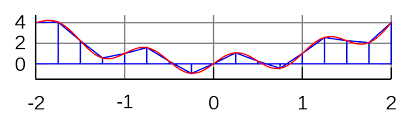
\includegraphics[scale=0.6]{num_int}
      \end{figure}
    \end{block}
  \end{itemize}
\end{frame}

\begin{frame}{Coupled Chemical System: Mathematical Description}
  \begin{columns}
    \begin{column}{.45 \textwidth}
      \begin{block}{Set of Elementary Reactions}
        \begin{equation*}
          \begin{gathered}
            A + B \rightarrow C \\
            B + C \rightarrow D \\
            D + E \rightarrow E + F \\
            F \rightarrow D + G \\
            E + G \rightarrow A   
          \end{gathered}
        \end{equation*}
      \end{block}
    \end{column}
    \begin{column}{.45 \textwidth}
      \begin{block}{Model Assumptions}
        \begin{itemize}
        \item $\bullet$ Many molecules: continuous and deterministic
        \item $\bullet$ Few molecules:\\ discrete and stochastic
        \end{itemize}
      \end{block}
    \end{column}
  \end{columns}
\end{frame}


\begin{frame}{Deterministic Framework}
  \begin{columns}
    \begin{column}{.45 \textwidth}
      \begin{block}{Set of Elementary Reactions}
        \begin{equation*}
          \begin{gathered}
            A + B \rightarrow C \\
            B + C \rightarrow D \\
            D + E \rightarrow E + F \\
            F \rightarrow D + G \\
            E + G \rightarrow A   
          \end{gathered}
        \end{equation*}
      \end{block}
    \end{column}
    \begin{column}{.45 \textwidth}
      \begin{block}{Computation}
        \begin{equation*}
          \begin{gathered}
            \frac{\partial [A]}{\partial t} = f_A\left([A], \dots [G]\right) \\
            \frac{\partial [B]}{\partial t} = f_B\left([A], \dots [G]\right) 
            \vdots\\
            \frac{\partial [G]}{\partial t} = f_G\left([A], \dots [G]\right)
          \end{gathered}
        \end{equation*}
      \end{block}
    \end{column}
  \end{columns}
\end{frame}

\begin{frame}{Stochastic Framework}
  \begin{columns}
    \begin{column}{.45 \textwidth}
      \begin{block}{Set of Elementary Reactions}
        \begin{equation*}
          \begin{gathered}
            R_1 + R^\prime_2 \xrightarrow{k_1} P_1 \\
            R_2 + R^\prime_2 \xrightarrow{k_2} P_2 \\
            R_3 + R_3^\prime \xrightarrow{k_3} P_3 + P_3^\prime 
          \end{gathered}
        \end{equation*}
      \end{block}
    \end{column} 
    \begin{column}{.45 \textwidth}
      \begin{block}{Propensity $k_i$}
        The probability that $i$-th reaction occurs
        in  $[0, dt]$ is
        $$k_i dt + o(dt)$$
        fixing molecules IDs a priori.
      \end{block}
    \end{column}
  \end{columns}
  \begin{block}{Reaction Rate $a_i$}
    The probability that $i$-th reaction occurs
    in  $[0, dt]$ is
    $$a_i dt + o(dt)$$
    with
    $$ a_i = k_i \cdot \# R_1 \dots \#R_n$$
  \end{block}
\end{frame}

\begin{frame}{Stochastic Framework}
  \begin{block}{Model Assumptions}
    \begin{itemize}
    \item $\bullet$ Molecules in solution $\implies$ No position $\implies$ States are multisets
      \begin{center}
        \begin{minipage}{.7 \textwidth}
          \begin{block}{State}
            $$ S = \left\{ \#M_1, \, \dots \#M_m \right\} $$
          \end{block}
        \end{minipage}
      \end{center}
      \vspace{1.pt}
    \item $\bullet$ Propensities are constant 
      \begin{center} 
       \begin{minipage}{.7 \textwidth}
          \begin{block}{Transition Probability}
            If $a_1$ reaction turns $S$ into $S^\prime$, then for each $t > 0$
            $$ \mathbb{P}\left(S^\prime, t + dt \,  \middle| \, S, t \right) = a_1dt + o(dt) $$
          \end{block}
        \end{minipage}
      \end{center}   
    \end{itemize}
  \end{block}
\end{frame}

\begin{frame}{How to Compute the Solution?}
  The model is finite state CTMC , solved exactly by
  \begin{block}{Master Equation}
    \begin{itemize}
    \item $\bullet$ One variable $p_S$ per state $S$
    \item $\bullet$ transition probabilities $\longrightarrow$ differential equations 
    \item $\bullet$ Exponential number of states $\implies$ intractable problem
    \end{itemize}
  \end{block}
  
  \begin{block}{Monte Carlo simulation}
    \begin{itemize}
    \item $\bullet$ Sample unbiased trajectories
    \item $\bullet$ Markov property simplifies computation
    \item $\bullet$ Gillespie's \textbf{Direct Method} and \textbf{First Reaction Method} 
    \end{itemize}
  \end{block}
\end{frame}

\begin{frame}{Reaction Times Distribution}
  Let $f:\left[0, +\infty\right) \longrightarrow \mathbb{R}^+$ density of $i$-th reaction 
  \begin{equation*}
    \left\{
    \begin{aligned}
      &f(0) = \frac{d}{dt} \mathbb{P}_i \left(dt \, \middle| \, S, 0 \right)= a_i\\
      &f(t + t_0) = \frac{f(t)}{1 - \int_0^{t_0} f(s)\, ds}         
    \end{aligned}\right.
    \implies f(t) = \left\{
    \begin{aligned}
        & a_i e^{-a_i t}   &\text{if } t \geq 0 \\
        &0 &\text{if } t < 0
    \end{aligned}\right.
  \end{equation*}
  \begin{block}{Exponential Distribution}
    \begin{itemize}
    \item $\bullet$ The density above corresponds to the r.v. $\Exp(a_i)$
    \item $\bullet$ $\Exp(a_1) \land \dots \land \Exp(a_n)$ is distributed as
      $\Exp\left(\sum_{i\leq n} a_i\right)$ 
    \item $\bullet$ If we 
    \end{itemize}
  \end{block}
\end{frame}

\begin{frame}{SNIPPETS}
  \begin{center}
    \begin{minipage}{.7 \textwidth}
      \begin{block}{Teorema}
        In quasi ogni torneo ogni vertice è un King.
      \end{block}
    \end{minipage}
  \end{center}
  \begin{columns}
    \begin{column}{.45 \textwidth}
      \begin{block}{Set of Elementary Reactions}
        \begin{equation*}
          \begin{gathered}
            R_1 + R^\prime_2 \xrightarrow{k_1} P_1 \\
            R_2 + R^\prime_2 \xrightarrow{k_2} P_2 \\
            R_3 + R_3^\prime \xrightarrow{k_3} P_3 + P_3^\prime 
          \end{gathered}
        \end{equation*}
      \end{block}
    \end{column} 
    \begin{column}{.45 \textwidth}
      \begin{block}{Propensity $k_i$}
        The probability that $i$-th reaction occurs
        in  $[0, dt]$ is
        $$k_i dt + o(dt)$$
        fixing molecules IDs a priori.
      \end{block}
    \end{column}
  \end{columns}
\end{frame}

\begin{frame}
  \begin{center}
    \Huge{Thank you for your attention.}
    \Huge{Questions?}
  \end{center}
\end{frame}

\end{document}

%%% Local Variables:
%%% mode: latex
%%% TeX-master: t
%%% End:
